\documentclass[11pt]{amsart}
\usepackage{geometry}                % See geometry.pdf to learn the layout options. There are lots.
\geometry{letterpaper}                   % ... or a4paper or a5paper or ... 
\usepackage{graphicx}
\usepackage{amssymb}
\usepackage{epstopdf}
\usepackage{pdfpages}
\usepackage{xcolor}
 \renewcommand{\abstractname}{Executive Summary}
 \definecolor{NeuroImageOrange}{RGB}{201,74,0}
\definecolor{SlateGrey}{RGB}{98,91,87}
\definecolor{Burgundy}{RGB}{146,15,15}
\usepackage[colorlinks=true, pdfstartview=FitV, linkcolor=NeuroImageOrange, 
            citecolor=blue, urlcolor=Burgundy]{hyperref}
\usepackage{fancyhdr}
\usepackage{multirow}
\usepackage[framemethod=TikZ]{mdframed}
\usepackage{caption}
\usepackage{subcaption}
\usepackage{wrapfig}
	\setlength\intextsep{0pt}
\DeclareGraphicsRule{.tif}{png}{.png}{`convert #1 `dirname #1`/`basename #1 .tif`.png}

\newenvironment{facts}[2][]{%
%    \refstepcounter{facts}
		\ifstrempty{#1}%
		% if condition (without title)
		{\mdfsetup{%
 		   frametitle={%
     		   \tikz[baseline=(current bounding box.east),outer sep=0pt]
       		 \node[anchor=east,rectangle,fill=teal!50]
       		 {\strut At A Glance%~\thefacts
		 };}
		    }%
		% else condition (with title)
		}{\mdfsetup{%
		    frametitle={%
		        \tikz[baseline=(current bounding box.east),outer sep=0pt]
		        \node[anchor=east,rectangle,fill=teal!50]
		        {\strut At A Glance%~\thefacts
		        :~#1};}%	
		    }%
		}%
		% Both conditions
		\mdfsetup{%
		    innertopmargin=10pt,linecolor=teal!50,%
		    linewidth=2pt,topline=true,%
		    frametitleaboveskip=\dimexpr-\ht\strutbox\relax%
		}
\begin{mdframed}[]\relax}{%
\end{mdframed}}

\title{DataHack: Understanding Police Misconduct}
\author{\href{http://isps.yale.edu/programs/policy-lab}{The Policy Lab} \& \href{https://www.law.yale.edu/centers-workshops/justice-collaboratory}{The Justice Collaboratory}}
\date{February, 2017}                                           % Activate to display a given date or no date

\begin{document}
\begin{center}
\includegraphics[scale=.5]{/Users/elizabethclarkpolner/Dropbox/PoliceComplaintNetworks/Misc/Administrative/Logos/YINS.jpg} \\
%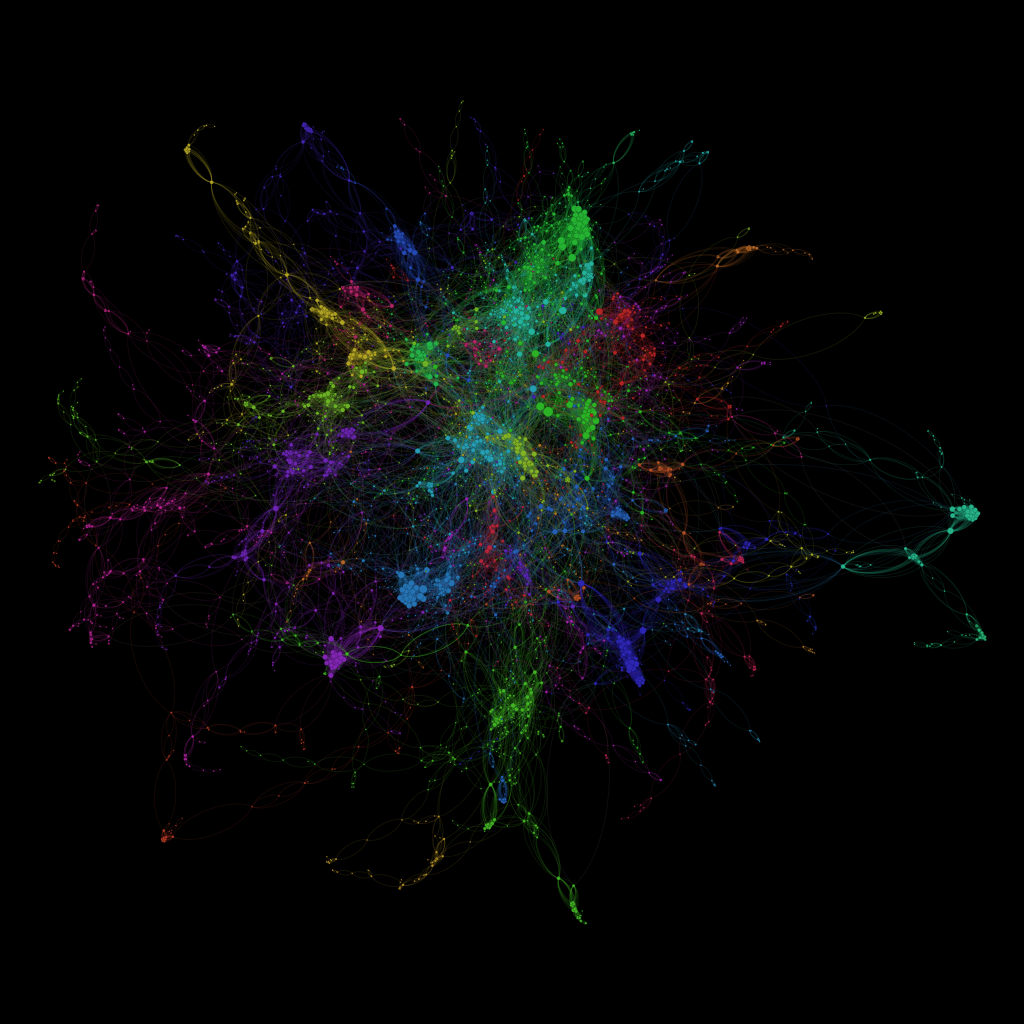
\includegraphics[scale=.05]{/Users/elizabethclarkpolner/Dropbox/PoliceComplaintNetworks/Projects/CPD_Initial/Analysis/Archived/29April2016/total-29april-v1.png}
\end{center} 

\maketitle
Every day a civilian is shot by a police officer in the United States. While rare as compared to other types of violence, the use of force by the police is of potentially greater importance: Force, utilized improperly or routinely, can erode trust between citizens and their government, prompt disengagement with the law, and shake the very foundation of our democracy.  

\begin{wrapfigure}{r}{0.35\textwidth}
  \begin{center}
    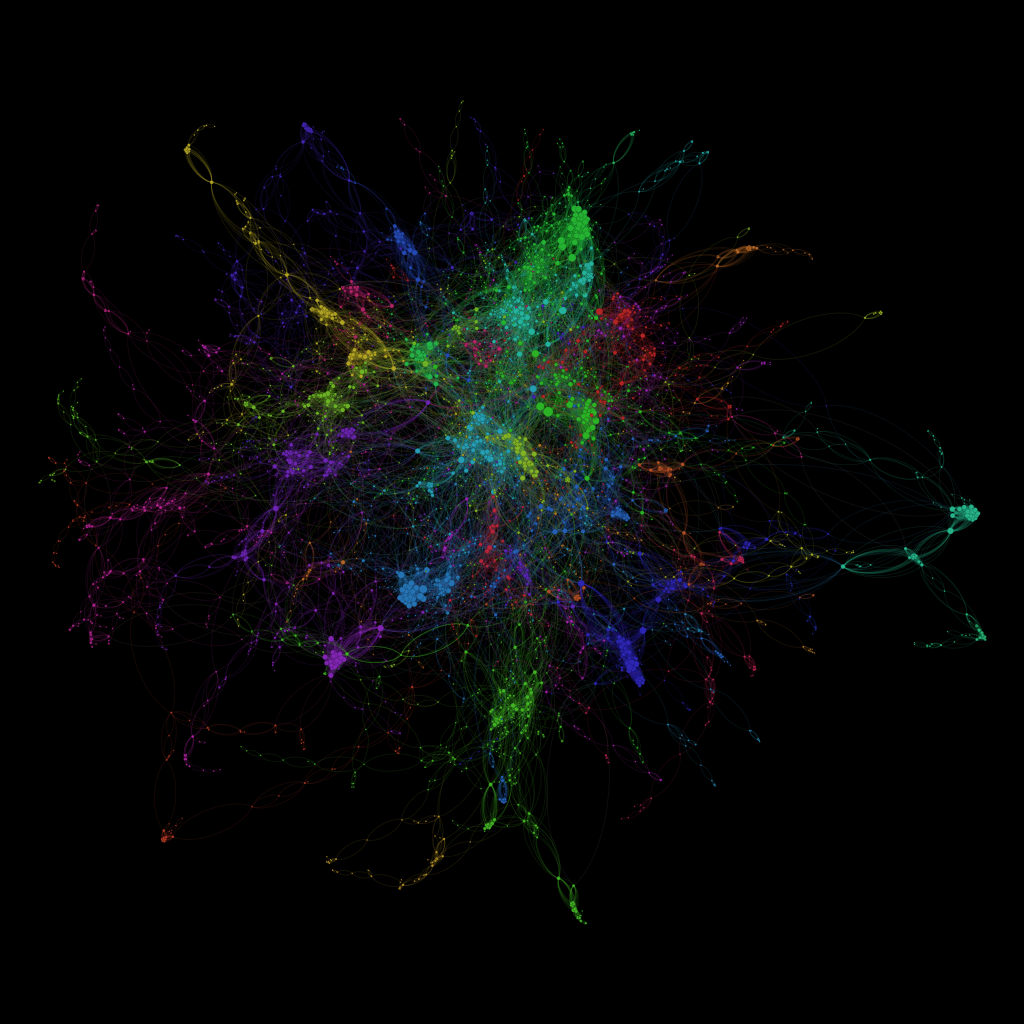
\includegraphics[width=0.3\textwidth]{/Users/elizabethclarkpolner/Dropbox/PoliceComplaintNetworks/Projects/CPD_Initial/Analysis/Archived/29April2016/total-29april-v1.png} \\
    \footnotesize{Communities of officers in Chicago}
  \end{center}
\end{wrapfigure}

Despite its importance, and the recent attention to police misconduct as a pressing social problem, there is still much we do not know about the phenomenon - including the rates of police misconduct, its distribution, and its root causes.  In large part, this is due to a lack of large-scale scientific inquiry, which itself results from a lack of data; neither police departments nor the government are compelled to compile and analyze incidents of police (mis)behavior in any systematic fashion. 

The recent series of high-profile shootings of unarmed citizens, however, has drawn the nation's gaze to this issue once again, and citizens, policy makers, and policing experts are mobilizing to uncover what data do exist.  One such repository comes from Chicago, IL, and contains records of allegations of police misconduct and investigations of police shootings dating back to 1971. The goal of this DataHack is to leverage this database to answer \href{https://www.whitehouse.gov/datadrivenjustice}{the White House's call} to develop smarter, more data-driven methods to understand and improve policing in the United States, and to reduce the use of force by officers.  Participants will have access to a database - compiled by \href{http://isps.yale.edu/programs/policy-lab}{The Policy Lab} and \href{https://www.law.yale.edu/centers-workshops/justice-collaboratory}{The Justice Collaboratory} at Yale Law School - containing more than 150,000 records of alleged police misconduct (built on reports made by both citizens and other police officers), as well as related datasets - including departmental and (anonymized) personnel records, maps of the city, and details as to its physical and political infrastructure. Hackers will be charged with uncovering actionable insights into the correlates -- and possible drivers -- of police misconduct, and will be evaluated based on the novelty, robustness, and scalability of their finished product, as well as the degree to which it highlights new conceptual threads as the foundation for future research. 

\vspace{.5in}
\begin{facts}[Possible Guiding Questions]
\textbf{Improving our Understanding of Police Misconduct}
	\begin{itemize}
	\item Is police misconduct a group or networked phenomenon? If so, what do police misconduct networks \textit{look} like? To what degree do police misconduct networks look and act like social and behavioral networks? For example, do people who work and train together, engage in misconduct together? 
	\item What are the behavioral and network-related correlates of police misconduct?  Are there particular characteristics by which we can differentiate officers who do and do not display more serious forms of misconduct?  
	\end{itemize}
\textbf{Improving our Prediction of Police Misconduct}
	\begin{itemize}
	\item How accurately can we predict future aggression by police officers?  Can we achieve top-shelf accuracy and efficiency in our predictions, but do so using models that can later be interrogated, so as to help policy makers and researchers better understand the underlying behavioral mechanisms at work (i.e. using something other than machine learning)? 
	\item How can we make all of these insights most useful to police departments, in real time? Can we develop visualization tools to aid police departments and citizens in understanding how misconduct concentrates within social networks? 
	\end{itemize}
\textbf{Improving our Study of Police Misconduct}
	\begin{itemize}
	\item How can we achieve the objectives listed above, but avoid over-fitting? These data come from one city (Chicago), within which some patterns may be idiosyncratic.  Can we build models that are likely to scale to other cities?  
	\item How can we estimate the scale and contents of missing data?  These allegations do not represent every incident of police misconduct -- rather, they reflect only those that were \textit{officially reported} - a time and energy intensive process, which also requires that citizens trust the police in the first place.  
	\end{itemize}
%}
\vspace{.1cm}
\end{facts}
\vspace{.5in}

\begin{center}

\includegraphics[scale=.07]{/Users/elizabethclarkpolner/Dropbox/PoliceComplaintNetworks/Misc/Administrative/Logos/policylab-final-yaleblue.jpg} \hspace{.4in} 
\includegraphics[scale=.6]{/Users/elizabethclarkpolner/Dropbox/PoliceComplaintNetworks/Misc/Administrative/Logos/Logo_YLS_JusticeCollaboratory.png}
\end{center}

\end{document}  